\chapter{Theory and Scope}
In this chapter, the scope of the study will be set. We dig into visual perspectives and define them by a continuum from ego-centric to exo-centric. Movements will be classified and discussed how to measure them. Eventually, a definition of mixed reality is provided. For a well designed study, these theoretical foundations are vital. If not indicated otherwise, the content is adopted from the book Motor Learning and Skills\cite{Schmidt2011}. 

\section{Visual Perspectives}
Wang and Milgram \cite{Wang2001} describe the perspectives on the centricity continuum, see figure~\ref{fig:ego-exo-cont}. On the most left-hand side of the continuum the ego-centric perspective is located. Ego-centric means that the anchor of the viewport is located inside the object to control - for simplicity, this object in question is referred to as an avatar. On the right-hand side the exo-centric perspective is located. This viewport anchor is a fixed point in the scene. The exo-centric perspective gives the user the possibility to examine the scene from a bird's-eye view. The movement or angle of the avatar has no influence on the viewports position or angle. The main difference is the so-called tether distance and the degree of freedom of the viewport. Milgram and Wang investigated on tethered viewports and define it as the distance between the eyes of the avatar and the viewport which is following the avatar. This describes the middle part of the continuum. Zero-distance viewport describes the ego-centric perspective. The longer the tether distance the more the perspective is located on the right of the continuum. They also distinguish between dynamic and rigid tethering relationships. A dynamic tethered viewport is controlled by the user in all six degrees of freedoms (DOF) while a rigid tethered viewport stands like a pole and can only be controlled in 3 DOF. Rigid tethered viewports are common in modern 3rd person computer games. In the next chapter, visual perspectives will be investigated in more detail.
\begin{figure}
	\centering
	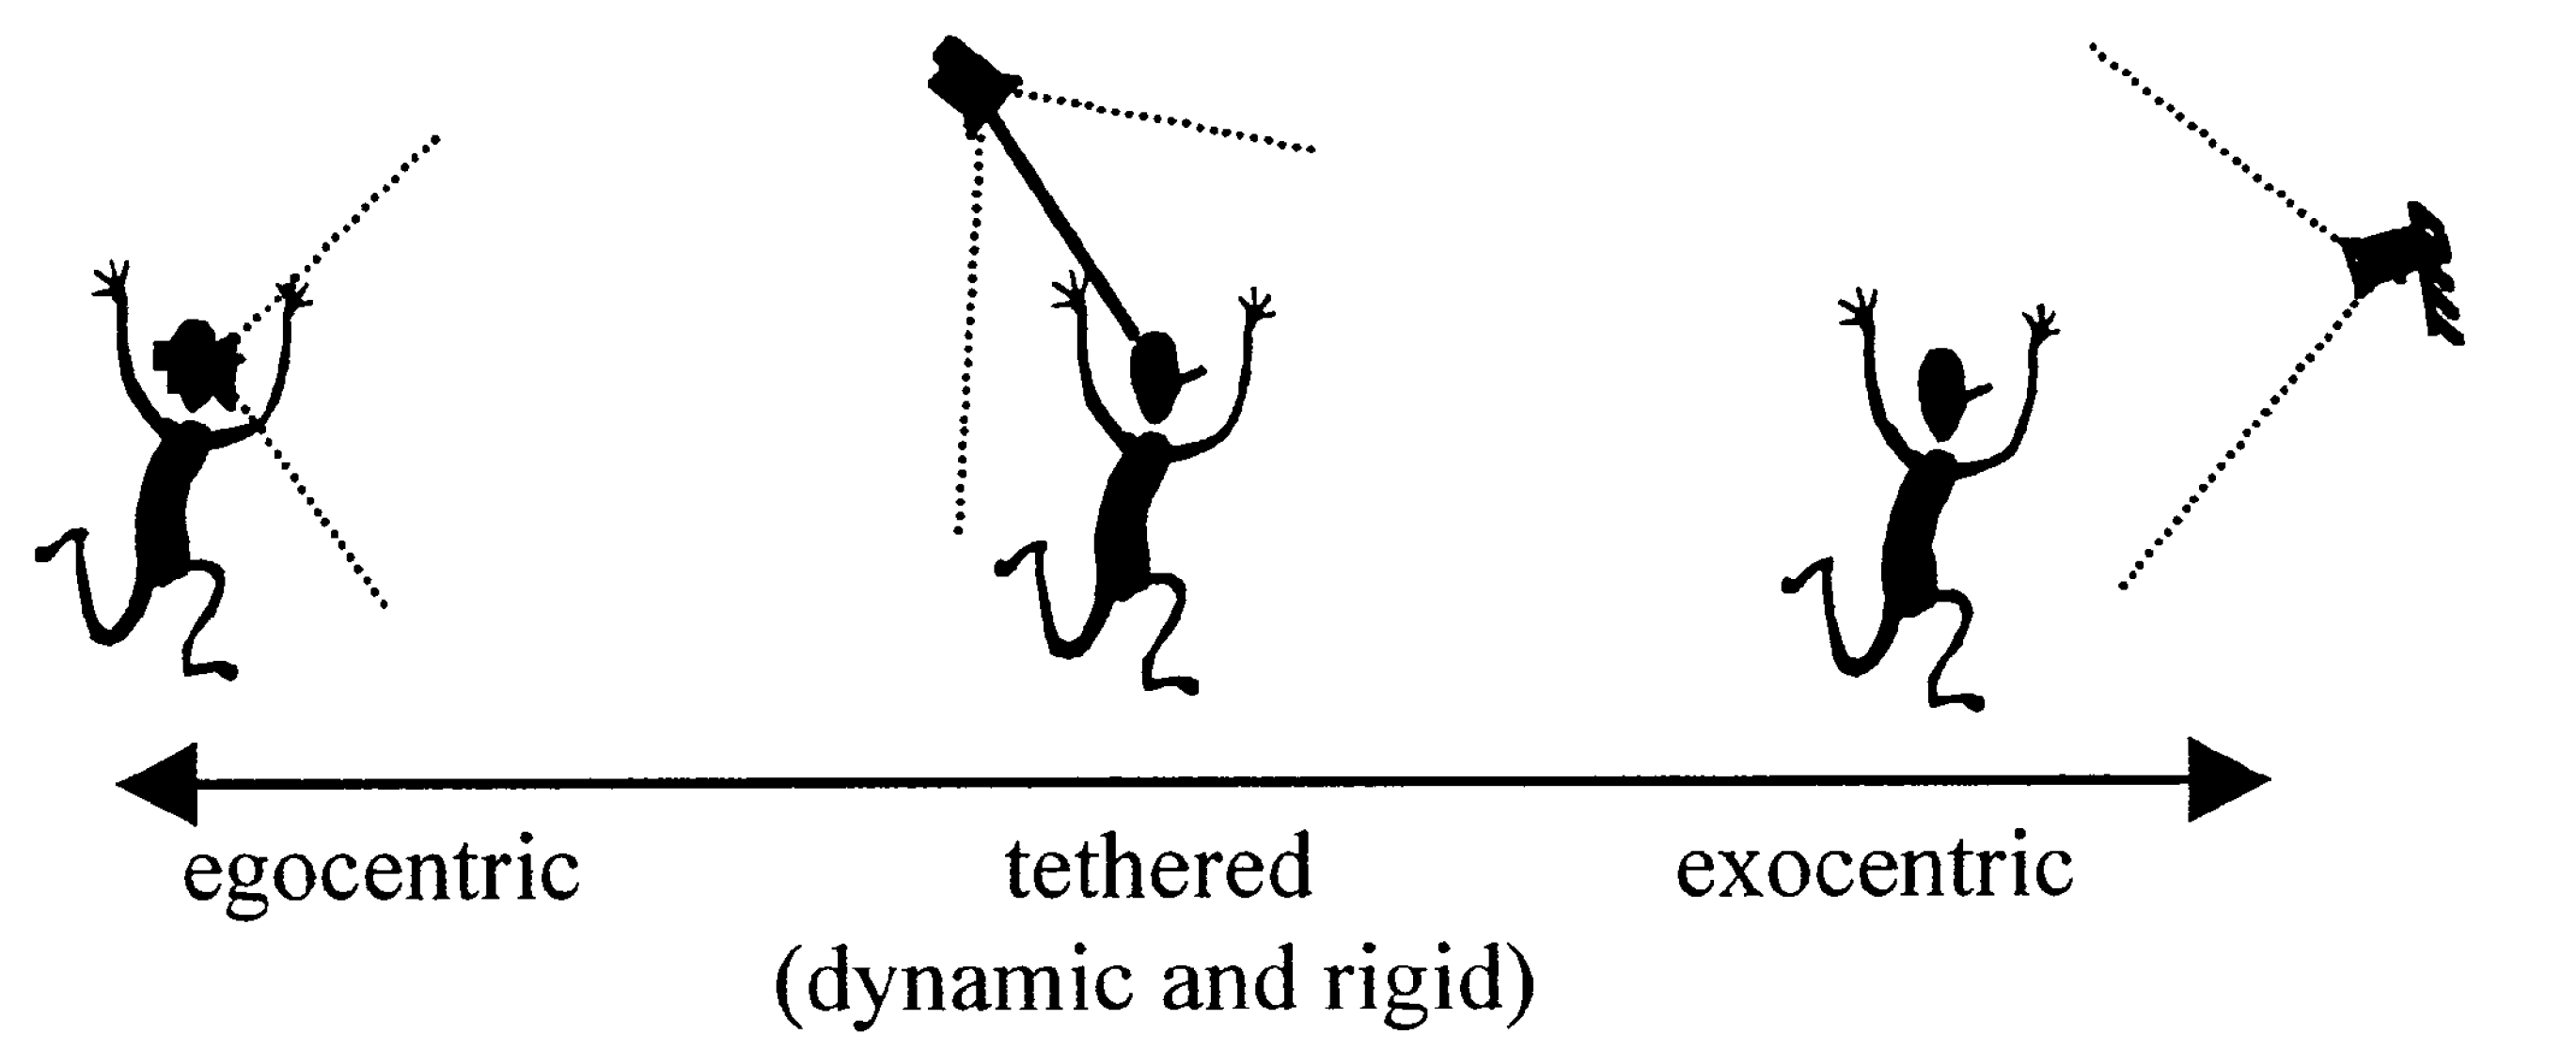
\includegraphics[width=1.0\textwidth]{img/ego_exo_continuum_bigger.PNG}
	\caption{Centricity continuum by Wang and Milgram \cite{Wang2001}.}
	\label{fig:ego-exo-cont}
\end{figure}

\section{Motor Learning}
\subsection{Learning Movements}
Motor learning is achieved through instruction, trying, imitation or a combination of them. Instructions can be written (see also figure~\ref{fig:laban} and further explanations in section~\ref{sec:measuringmovements}), visual or verbal. Visual or verbal instruction include a trainer, teaching the student movements. In this case, verbal and physical feedback also plays a role in the learning process. The process of motor learning is divided into three parts. In the beginning of learning a technique, the student starts in the \textit{cognitive} stage. In this stage, the students tries to figure out what to do to achieve the task. For this, high cognitive activity is required and strategies needs to be evaluated. The student's performance increases dramatically and is larger than in any other stage, but also inconsistent. The use of instructions and other training techniques are most effective. The next stage is called the \textit{associative} stage. It begins when the student has determined the most effective way of doing the task. Performance increases more gradually but becomes more consistent. In the last \textit{autonomous} stage, the performer gains proficiency and other simultaneous happening tasks are less likely to interfere. 
\begin{tcolorbox}[colback=red!30!white]
Since the use of training methods are most effective in the \textit{cognitive} stage and the performance gain is highest in the \textit{cognitive stage}, tasks in this stage are best suited for the study.
\end{tcolorbox}

%maybe sth about time and money

\subsection{Movement Classification}
Movements can be classified. There are two common classification schemas. The first one is based on the particular movements performed and is divided into \textit{discrete}, \textit{continuous} and \textit{serial movements}, compare figure~\ref{fig:movements_cont}. The second one is based on perceptual attributes of the task and is divided into \textit{open} and \textit{closed skills}, compare figure~\ref{fig:skills_cont}. Both classification are represented by a continuum.

\subsubsection{Discrete, Continuous and Serial Movements}
\begin{figure}[h]
	\centering
	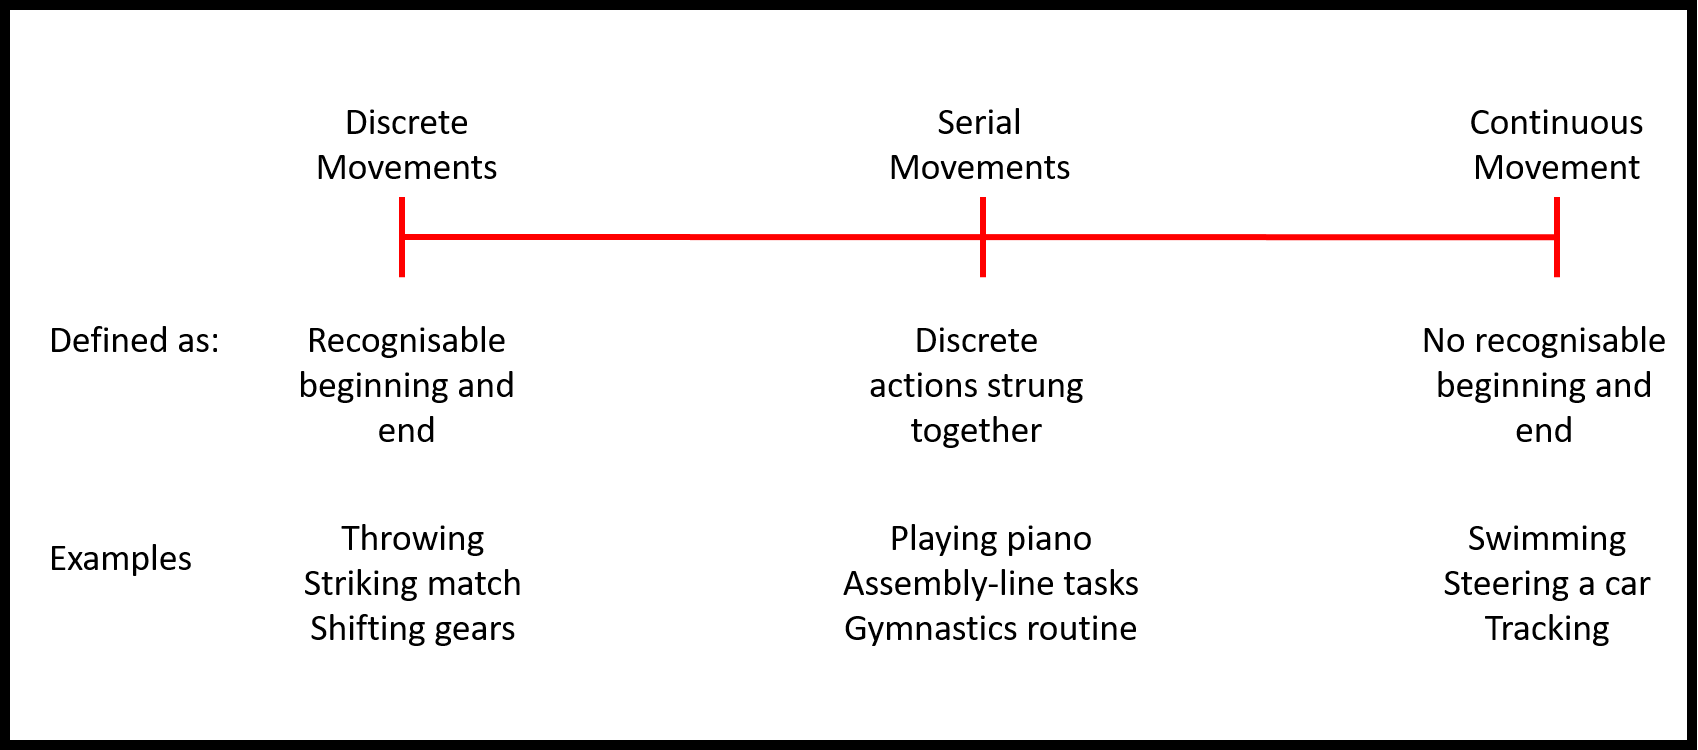
\includegraphics[width=1.0\textwidth]{img/movement_classification.png}
	\caption{Continuum of movement classification based on the movement itself, redrawn from \cite{Schmidt2011}.}
	\label{fig:movements_cont}
\end{figure}
\textit{\textbf{Discrete movements}} are located on the one end of the continuum. These are movements with a recognisable beginning and end. The end of a discrete movement is defined by the task itself and can be very rapid like blinking or longer like undersigning. Examples are kicking a ball, shifting gears in a car or striking a match.\\
\textit{\textbf{Continuous movements}} are located on the other end of the continuum. These movements do not have a recognisable beginning or end. The behaviour continues till the movement arbitrarily stops. Continuous tasks tend to be longer than discrete tasks. Examples are swimming, running or steering a car.\\
\textit{\textbf{Serial movements}} are located in the middle part of the continuum. Following the nature of a continuum, these movements are neither discrete nor continuous. They can consist of smaller movements tied together. Furthermore, serial movements can be rather long but are not stopped arbitrarily. Serial tasks can be seen as many discrete tasks strung together and the order (and sometimes timing) is important. Examples are starting a car or preparing and lighting a wood fireplace.\\
The nature of \textit{continuous movements} is having no recognizable beginning and end. This makes it hard to describe a distinctive task for a study design. While \textit{discrete movements} are too short for a proper task, \textit{serial movements} are most suitable for a study task.\\
\begin{tcolorbox}[colback=red!30!white]
\textit{Discrete movements} are too short for a proper evaluation. Because of the nature of having no recognisable beginning and end, \textit{Continuous movements,} also seems not to be suitable as a task in a study. Furthermore, in chapter 3 we will see that most researchers use \textit{serial movements} as study task. Because of this, the scope is set for serial movements as study task.
\end{tcolorbox}

\subsubsection{Open and Closed Skills}
\begin{figure}[h]
	\centering
	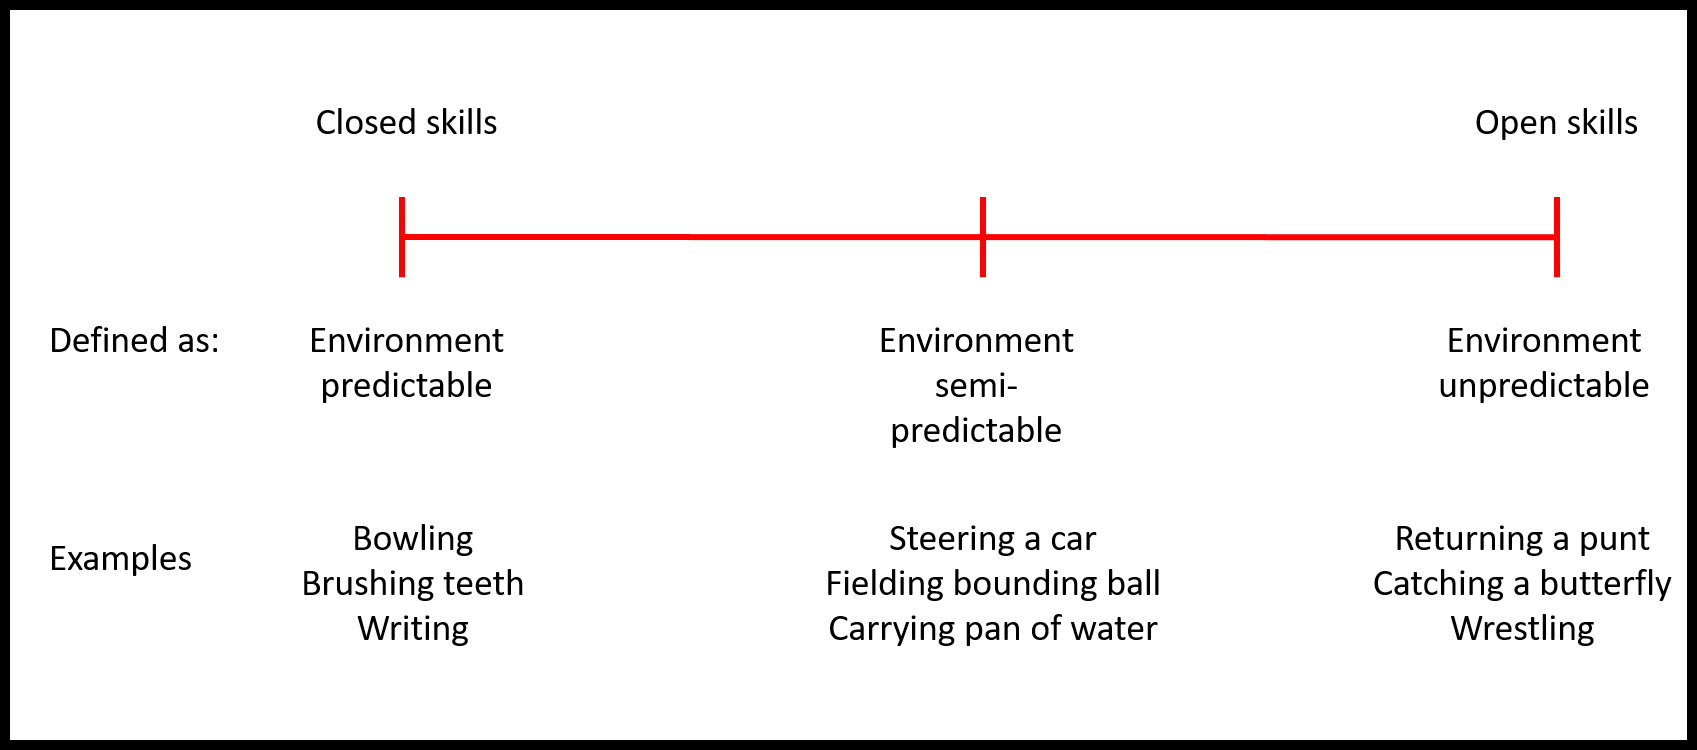
\includegraphics[width=1.0\textwidth]{img/movement_classification2.png}
	\caption{Continuum of movements classification based on perceptual attributes, redrawn from \cite{Schmidt2011}.}
	\label{fig:skills_cont}
\end{figure}
\textit{\textbf{Open skills:}} The environment is unpredictably changing. The performer cannot plan his activity effectively in advance. Own movements depend on the environment. For example, if an ice hockey player shoots a puck, his movement dependents on the movement of the keeper. Another example is driving on a freeway. The driver needs to adjust his driving dependent on the behaviour of other cars. Success in open skills is largely determined by the extent to which an individual can adapt the planned motor behaviour to the changing environment.\\
\textit{\textbf{Closed skills:}} The environment is predictable, mainly because it is stable. This means that the performer can plan his activity. Examples are bowling, archery or singing. To evaluate only the motor learning and not environmental influences the study is conducted in a controlled environment in a laboratory. Thus only \textit{closed skills} are taken into consideration.\\
\begin{tcolorbox}[colback=red!30!white]
This work aims to evaluate the influence of the visual perspective on motor learning, not how well students can react to unforeseen changes in the environment. Therefore, the scope is set to \textit{closed skills}.
\end{tcolorbox}


%since open skills  seems to require rapid adaptions to a changing environment and closed skills require a very stable performances in a predictable environment questions are raised about the method of training, do different individuals perform better in in one of these skill classes. to overcome these question the focus of this seminar is on discrete movement tasks and closed skills. $->$ see study \todo + citations



\begin{comment}
Kwon et al. \cite{Kwon2005} \todo 
\begin{itemize}
\item K. Hachimura, K. Takashina, and M. Yoshimura, “Analysis and
Evaluation of Dancing Movement Based on LMA,” Proc. IEEE Int’l
Workshop Robots and Human Interactive Comm., pp. 294-299, 2005.
\item M. Yoshimura, N. Mine, T. Kai, and L. Yoshimura, “Quantification    of Characteristic Features of Japanese Dance for Individuality Recognition,” Proc. IEEE Int’l Workshop Robot and Human Interactive Comm., pp. 193-199, Sept. 2001.
\item G. Qian, F. Guo, T. Ingalls, L. Olson, J. James, and T. Rikakis, “A    Gesture-Driven Multimodal Interactive Dance System,” Proc. IEEE    Int’l Conf. Multimedia and Expo (ICME ’04), pp. 1579-1582, June    2004.
\item D.Y. Kwon and M. Cross, “Combining Body Sensors and Visual
Sensors for Motion Training,” Proc. ACM SIGCHI, pp. 94-101,    2005.
\item vr dance trainer
\end{itemize}
\end{comment}


\subsection{Measuring Movements}
\label{sec:measuringmovements}
%Welche messmethoden gibt es um bewegungen zu messen
To measure a movement and matching it to a given motion is not a trivial task. Since e.g. dancing is a purely physical task, movements must be recognised, digitalised and judged. One approach is to use an analogue description for dancing and translate them into the digital world. Choensawat\cite{Choensawat2015} began with Rudolph von Laban - a professional dancer. Von Laban developed a broadly used dance notation. His work lead to the \textit{Laban Movement Analysis} with which human movements could be quantized\footnote{Brockhaus, Rudolf Laban. \hyperlink{http://www.brockhaus.de/ecs/enzy/article/laban-rudolf}{http://www.brockhaus.de/ecs/enzy/article/laban-rudolf (accessed 2018-10-25)}}. There are four main components to systematically describe movements in the \textit{Laban Movement Analysis}: body, effort, shape and space. Each component can describe movements independently or combined. Hachimura et al. \cite{Hachimura2004} used the methodology of \textit{Laban Movement Analysis} and adopted it for digital movements.\\
Yoshimura et al. \cite{Yoshimura2006} followed a similar approach from another dance movement description theory called \textit{furi}. \textit{Furi} is described by four so-called \textit{indices}: \textit{kamae}, \textit{jyu-shin}, \textit{koshi}, \textit{uchiwa}. Yoshimura et al. map these indices to concrete markers on the body of a performer. Qian et al. \cite{Qian2005} developed a gesture recognition system for performing arts. To match the motions ten body parts were defined: head, torso, upper arms, forearms, upper legs and lower legs. For each body part, the Mahalanobis distance is calculated to an ideal point. The Mahalanobis distance describes the distance between point \textit{p} and distribution \textit{D}.\\
To measure a movement, a common approach is to measure a single point on the subjects body repeatedly and then calculate an overall score, measuring how accurate the movement was. In literature, three main categories of those point measures are listed: \textit{error of a single subject}, \textit{measures of time and speed} and \textit{measures of movement magnitude}.
\begin{tcolorbox}[colback=red!30!white]
As chapter 3 will show, \textit{error of a single object} and \textit{measures of time and speed} is most commonly used and is most promising to generate the date in question. For this reason, these two measures will be used to evaluate the movements in the study proposed in chapter 4. \textit{Measures of movement of magnitude} suit not for the evaluation, because of the nature of the task which is described in chapter 3.
\end{tcolorbox}
\begin{figure}
	\centering
	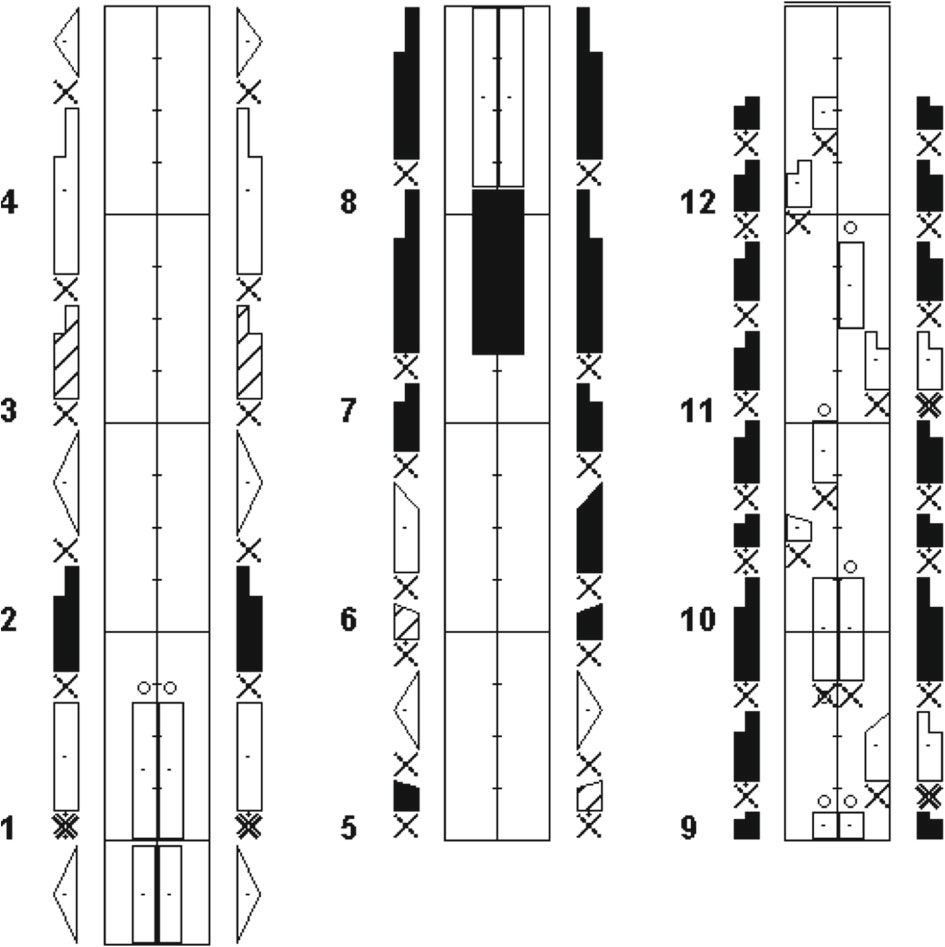
\includegraphics[width=0.5\textwidth]{img/laban.png}
	\caption{Laban notation. Generated through automatic movement interpretation by Choensawat \cite{Choensawat2015}.}
	\label{fig:laban}
\end{figure}

\subsubsection{Measures of Error for a Single Subject}
Measures of error for a single subject represent the degree to which the target movement was missing. A target can be to perform an act at a particular time (timestamp), move with a certain force (amount of force) or hit a spatial target (a point in spatial volume). The attribute of the target serves as the variable in question. The error itself describes the distance - regarding the dimension - from the target. The following list gives an insight into the most important error measures.
\begin{itemize}
	\item \textbf{\textit{Constant Error}} describes the average error between the actual accuracy and the target. Means, in average the performer missed the target by CE.
	\begin{equation}
	\label{eq:constanterror}
	CE=\frac{\sum_i(x_i-T)}{n}
	\end{equation}
	with $x_i$: score, $n$: number of values, $T$: target value.
	\item \textbf{\textit{Variable Error}} measures the inconsistency in movements. The more consistent the movements, the smaller $VE$. $VE$ does not depend on whether or not the subject was close to the target.
	\begin{equation}
	VE=\sqrt{\frac{\sum(x_i-T)^2}{n}}    
	\end{equation}
	with $x_i$: score, $n$: number of values, $T$: target value.
	\item \textbf{\textit{Total Variability}} describes the total variability around a target. The combination of VE and CE represents the total amount of spread around the target. It is an overall measure how successful the subject was in achieving the target.
	\begin{equation}
	E=VE^2+CE^2=\sqrt{\frac{\sum(x_i-T)^2}{n}}
	\end{equation}
	with $x_i$: score, $n$: number of values, $T$: target value.
	\item \textbf{\textit{Absolute Error}} is a measure of the overall accuracy in performance.
	\begin{equation}
	AE=\frac{\sum|x_i-T|}{n}
	\end{equation}
	with $x_i$: score, $n$: number of values, $T$: target value.
	\item \textbf{\textit{Absolute Constant Error}} is the absolute value of $CE$. Because of negative and positive values can cancel each other out
	\begin{equation}
	ACE = |CE|
	\end{equation}
\end{itemize}



\subsubsection{Measures of Time and Speed}
\label{section:timeandspeed}
The basic idea of time and speed measures is, that a performer who can accomplish more in a given amount of time or who can accomplish a given amount of behaviours in less time is more skilful. Measures here are
$\frac{time}{unit}$ or $\frac{units}{time}$.\\
The two most common examples are \textit{reaction time} (RT) and \textit{movement time} (MT). Reaction time describes the amount of time between a stimulus and the regarding start of a movement. This time span is important for two reasons. First, RT has high validity for real-life tasks. Secondly, RT measures the time taken for mental events like stimulus processing or decision making.\\
\textit{Movement time} is the time interval between the end of the RT phase, meaning the start of the response, and the completion of the movement. The sum of RT and MT is called \textit{response time}.
%line{reaction time} (RT): can also be a performance measure. a measure of time from the arrival of a sudden and unanticipated signal to the beginning of the response. 

\subsubsection{Measures of Movement Magnitude}
To measure skill, the produced magnitude of behaviour can be used. E.g. the distance a discus is thrown. A famous example is the "ski simulator". Rubber bands hold a plate centred between two poles. The magnitude, in this case, is the dislocation of the board from the centre by using full-body movements. As described, this measure can not be used for the task used in the proposed study design, thus only described in short.

\section{Mixed Reality}
Already in 1994 Milgram and Kishinho \cite{Milgram1994} defined the Mixed Reality continuum for displays, see figure~\ref{fig:MRcont}. On the most left-hand side, the real world is located. On the right-hand side the purely digital world is located. The more we move from the left to the right, the more of the real world is replaced with digital elements. Respectively, starting from a purely digital environment and moving on the continuum to the left, the more of the digital environment is replaced by real-world elements.
\begin{figure}
	\centering
	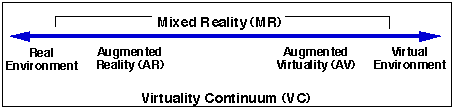
\includegraphics[width=1.0\textwidth]{img/milgram_continuum.png}
	\caption{Mixed reality continuum by Milgram et al. \cite{Milgram1994}.}
	\label{fig:MRcont}
\end{figure}
In virtual reality, the view on the real world is completely blocked. Common devices are e.g. the Oculus Rift or HTC Vive. Augmented reality can be realised by optical see-through devices like the Microsoft HoloLens. Seeing the own body during motor learning seems to be intuitively the best way to maintain the perception of their own body.
\begin{tcolorbox}[colback=red!30!white]
But for the following reason the scope is set to VR: AR technology is still limiting, especially because of their small field of view, which can influence guiding negatively \cite{Katzakis2017}. Video see-through provides a larger field of view but also has limiting aspects like latency and distortion. In this case, the representation of the own body needs to be maintained by using motion capturing and rendering on the position of the own body.
\end{tcolorbox}

\section{Summary}
This chapter provides theoretical foundations needed for the planned research in the field of perspectives and motor learning. Furthermore, the scope of the research was set. \textbf{Measures for single error} will be applied in the study. The task will be a \textbf{serial task} and also only \textbf{closed skills} will be trained. Eventually, the study will take place in \textbf{virtual reality}.